\section{Experiments}

In this section, we discuss the experiments settings of ConFu. We report the result of ConFu and other baseline methods on two datasets. To further demonstrate the effectiveness of ConFu, we use TSNE \cite{van2008visualizing} to visualize query embedding and product embedding by models. Case study is also performed to show how ConFu solves problems in our scenario.

\subsection{Datasets}

In order to demonstrate the effectiveness of ConFu, we perform experiments on two PSR datasets. 

\subsubsection{MMMPS}
% \sansa{\sout{re-consider the name}}
MMM Product Search (MMMPS or MMM) is the dataset from our own life-service scenario and will be released. MMMPS dataset is a binary dataset and for each query-product pair, the corresponding label is relevant (1) or irrelevant (0). For this data set, we use Area Under the receiver operating characteristic Curve (AUC) to evaluate the performance of different models. 

\begin{table}[th]
\setlength{\tabcolsep}{2.8pt}
\begin{threeparttable}[b]
  \caption{Dataset statistics of MMMPS dataset}
  \label{tb:dataset}
  \centering
  \begin{tabular}{cccccc}
    \toprule
    \# training  & \# dev  & \# test  & \# 1st cate. & \# 2nd cate. & \# 3rd cate. \\
    \midrule
    100k & 10k & 19,959 & 27 & 199 & 1,577 \\
    % \small{BH} & 31k & 5k & 2632 & 4 & no \\
    % \small{FG} & 28k & 3k & 1065 & 4 & no \\
    \bottomrule
  \end{tabular}
  \begin{tablenotes}
    \item[1] The hierarchical taxonomy of MMMPS dataset is a three-level tree-structured taxonomy.
  \end{tablenotes}
  \end{threeparttable}
\end{table}

Statistics of MMMPS dataset is listed in Table \ref{tb:dataset}. In MMMPS dataset, there are 119,845 different kinds products from 1,577 different categories, which means most products appear few times in the dataset and the ratio of unique products in the dataset can reach around 92\%. MMMPS covers most product categories we can see in all kinds of shops in our daily life, which makes it a challenging dataset. For most queries, their connected concepts like synonyms and hypernyms in KG are also provided.

\subsubsection{WANDS}

WANDS dataset \cite{chen2022wands} is also a product search relevance dataset released by wayfair. In this data set, hierarchical category and product class are provided for products. Query class is provided for query. The hierarchical categories and product/query classes can be taken as KG of this dataset. There are three labels in this dataset: Exact, Partial and Irrelevant. In order to make it consistent with MMMPS dataset, we drop the Partial labels and make it a binary class dataset, denoted as WANDS-binary. We also drop duplicate data and split data into training set, dev set and test set. The evaluation metric of WANDS-binary dataset is AUC. Note that although problems we claimed are not significant in this dataset, it is still a good dataset to evaluate and analyze different methods.

% NDCG@10
\subsection{Baselines}
% \sansa{need to add baselines, too weak}
\subsubsection{Sentence-BERT}
Sentence-BERT (SBERT) \cite{reimers2019sentence} is a two-tower or bi-encoder structure model, which is widely adopted in industry scenarios including ours. The bi-encoder structure is very efficient due to its ability to embed query and product separately.

\subsubsection{SBERT+KGP}
One of the most direct and common approaches to utilize KG is to concatenate the knowledge in text form from KG on the original text \cite{bian2021benchmarking, weijie2019kbert}. In PSR task, we implement such a method by concatenating Knowledge Graph Path (KGP) of query and product. In SBERT+KGP, knowledge in KG of specific query and product is concatenated to query and product respectively.

\subsubsection{SBERT+KGE}
Another commonly used method to utilize KG is fusing knowledge in KG through Knowledge Graph Embedding (KGE), which shows competitive performance in \cite{luo2021alicoco2, huang2019knowledge, sun2018recurrent}. The advantage of KGE is that it concerns the overall structure of KG. Thus, we adopt this method as one of our baseline methods. In SBERT+KGE, KGE of nodes in KG trained by PairRE \cite{chao-etal-2021-pairre} is concatenated to the embedding of query and product.

% \zelin{missing citation here. we should claim that KGP and KGE are commonly used methods, which shows competitive performance in ... paper}

\subsection{Implementation Details}
 % We deploy all experiments on Nvidia V100 32G GPU.
 BERT-related models are initialized from the pretrained Google BERT-base (Chinese) and tuned with 2e-5 learning rate and 128 batch size. The optimizer is AdamW. In model selection, for each model, we trained enough epochs for each model and select the best performing checkpoint on the dev set to be the final trained model. Each experiment is repeated three times with different random seeds and corresponding scores are averaged.

\subsection{Overall Results}
% \sansa{As for the main table, you'd better merge Table \ref{tb:mt} and Table \ref{tb:wands}.}

The overall experiment results on two datasets are displayed in Table \ref{tb:mt}. Result on both dev set and test set is reported.

% Table \ref{tb:mt} is the experiment results on our own MMMPS dataset and Table \ref{tb:wands} is the experiment results on WANDS-binary dataset.

% The best results are bolded, the best baseline results are starred.

\begin{table}[!th]
  \centering
  \setlength{\tabcolsep}{1pt}
  \begin{threeparttable}
  \caption{The AUC score of our \textit{ConFu} framework and other baseline methods on MMMPS and WANDS-binary. KGP and KGE stands for concatenating Knowledge Graph Path and Knowledge Graph Embedding respectively. Query/product only means only Query/Product Contrastive Knowledge Fusion is adopted in ConFu. }
  \label{tb:mt}
  \centering
  \begin{tabular}{l|l|l|l|l}
    \toprule
    Methods & ${MMM}_{dev}$  & ${MMM}_{test}$ & ${WANDS}_{dev}$  & ${WANDS}_{test}$ \\
    \midrule
    SBERT & 0.764 & 0.765 & 0.955 & 0.960 \\
    SBERT+KGP & 0.768 & 0.771 & 0.956 & 0.962 \\
    SBERT+KGE & 0.756 & 0.756 & 0.958 & 0.962 \\
    \midrule
    \textit{ConFu}  & 0.800 & 0.800 & 0.980 & 0.981  \\
    \textit{ConFu (query only)}  & 0.771 & 0.769 & 0.982 & 0.984 \\
    \textit{ConFu (product only)} & 0.779 & 0.779 & 0.927 & 0.927 \\
    \textit{ConFu+KGP} & 0.797 & 0.793 & 0.944 & 0.947  \\
    % \textit{ConFu-KGP-QCL}  & 0.787 & 0.785 \\
    % \textit{ConFu-KGP-PCL}  & 0.769 & 0.768 \\
    \textit{ConFu+KGE} & 0.795 & 0.795 & 0.981 & 0.982 \\
    % \textit{ConFu-KGE-QCL} & 0.767 & 0.768 \\
    % \textit{ConFu-KGE-PCL} & 0.792 & 0.791 \\
    \bottomrule
  \end{tabular}
  % \begin{tablenotes}
  %   \item[1] MMM means MMMPS dataset.
  % \end{tablenotes}
  \end{threeparttable}
\end{table}

\subsubsection{Results on MMMPS}

On MMMPS dataset, our experiment results illustrate the effectiveness of ConFu compared with vanilla SBERT, SBERT+KGP and SBERT+KGE. According to the experiment result of SBERT+KGP and SBERT+KGE, we can see that simply concatenating KGP or KGE can bring limited improvement on model performance. With contrastive learning, ConFu can effectively inject knowledge in KG into PSR model. Specifically, QCKF and PCKF in ConFu can complement each other in such case where both query and product are ambiguous. Note that though ConFu can also be applied on Model+KGP or Model+KGE, our experiment result shows that ConFu only is sufficient for effective knowledge fusion.

Besides, we also perform T-test on our results with a critical value 0.05 and the following conclusions can be made:

\begin{enumerate}
  \item ConFu and its variants (ConFu+KGP and ConFu+KGE) are significantly better than baseline methods with p-value 0.004, 0.016 and 0.025 on test set respectively, which demonstrates the effectiveness of ConFu.
  \item Though ConFu (query only) and ConFu (product only) cannot significantly outperform baseline methods, they can complement each other well and so that ConFu can achieve significant improvement.
  \item Confu, ConFu+KGP and ConFu+KGE have similar performance, which means ConFu is sufficient for effective knowledge fusion.
\end{enumerate}

% Besides, ConFu is orthogonal to other knowledge fusion methods and it can be applied on other knowledge fusion methods to enhance model's understanding of query and product. 


% % this is the original result of WANDS ---------------------------------
% \begin{table}[!th]
%   \centering
%   \setlength{\tabcolsep}{9pt}
%   \begin{threeparttable}
%   \caption{The NDCG@10 score of our \textit{ConFu} framework and other baseline methods. The best results are bolded, the best baseline results are starred.}
%   \label{tb:mt}
%   \centering
%   \begin{tabular}{l|l|l}
%     \toprule
%     Methods & Dev Set & Test Set \\
%     \midrule
%     Sentence-BERT & 0.913 & 0.910 \\
%     Sentence-BERT-KGP & 0.919 & 0.917$^*$ \\
%     Sentence-BERT-KGE & 0.915 & 0.910 \\
%     \midrule
%     \textit{ConFu} & 0.919 & 0.916 \\
%     \textit{ConFu (query only)} & \textbf{0.932} & \textbf{0.929} \\
%     \textit{ConFu (product only)} & 0.920 & 0.914 \\
%     \textit{ConFu-KGP} & 0.917 & 0.912 \\
%     \textit{ConFu-KGE} & 0.923 & 0.917 \\
%     \bottomrule
%   \end{tabular}
%   % \begin{tablenotes}
%   %   \item[1] ...
%   % \end{tablenotes}
%   \end{threeparttable}
% \end{table}
% % this is the original result of WANDS ---------------------------------

% \begin{table}[!th]
%   \centering
%   \setlength{\tabcolsep}{15pt}
%   \begin{threeparttable}
%   \caption{The AUC score of our \textit{ConFu} framework and other baseline methods on WANDS-binary dataset. KGP and KGE stands for concatenating Knowledge Graph Path and Knowledge Graph Embedding respectively. Query/product only means only Query/Product Contrastive Knowledge Fusion is adopted in ConFu. }
%   \label{tb:wands}
%   \centering
%   \begin{tabular}{l|l|l}
%     \toprule
%     Methods & Dev Set & Test Set \\
%     \midrule
%     SBERT & 0.955 & 0.960 \\
%     SBERT+KGP & 0.956 & 0.962 \\
%     % Sentence-BERT-KGP-lastcate & 0.963 & 0.970 \\
%     SBERT+KGE & 0.958 & 0.962 \\
%     \midrule
%     \textit{ConFu} & 0.980 & 0.981 \\
%     \textit{ConFu (query only)} & 0.982 & 0.984 \\
%     \textit{ConFu (product only)} & 0.927 & 0.927 \\
%     \textit{ConFu+KGP} & 0.944 & 0.947 \\
%     % \textit{ConFu-KGP-QCL}  & \textbf{0.984 }& \textbf{0.986 }\\
%     % \textit{ConFu-KGP-PCL}  & 0.900 & 0.903 \\
%     % \textit{ConFu-KGP-lastcate} & 0.967 & 0.969 \\
%     % \textit{ConFu-KGP-lastcate-QCL}  & \textbf{0.992}& \textbf{0.993}\\
%     % \textit{ConFu-KGP-lastcate-PCL}  & 0.937 & 0.939 \\
%     \textit{ConFu+KGE} & 0.981 & 0.982 \\
%     % \textit{ConFu-KGE-QCL}  & 0.982 & 0.984 \\
%     % \textit{ConFu-KGE-PCL}  & 0.934 & 0.932 \\
%     \bottomrule
%   \end{tabular}
%   % \begin{tablenotes}
%   %   \item[1] ...
%   % \end{tablenotes}
%   \end{threeparttable}
% \end{table}

\subsubsection{Results on WANDS-binary}

On WANDS-binary dataset, ConFu can also outperforms baseline methods. However, one difference is that PCKF fails on WANDS-binary dataset and the performance gain is basically contributed by QCKF. One possible reason why PCKF of ConFu does not work on WANDS-binary is that product name in WANDS-binary has already contained information in taxonomy and products in each categories share similar names, and external knowledge from Knowledge Graph is not that informative and necessary enough. For instance, the KGP of products ``totham rocking chair'', ``ossu outdoor rocking chair with cushions'', ``sonnenberg rocking chair'' and ``fordyce rocking chair'' is ``Outdoor / Outdoor \& Patio Furniture / Outdoor Seating \& Patio Chairs / Patio Seating / Patio Rocking Chairs \& Gliders'' and ``rocking chair'' appears in all four products. This point can also be demonstrated by product embedding visualization in the following section. Additionally, WANDS-binary dataset is simpler than MMMPS dataset as MMMPS dataset contains more kinds of products and more fine-grained Chinese introduces more ambiguity while WANDS-binary dataset contains only Furniture \& Home products. Thus, additional PCKF can easily cause overfitting on product embedding learning with coarse-grained taxonomy on WANDS-binary with well self-separated products. Different from product, query in WANDS-binary is usually short and needs more knowledge, so QCKF can effectively improve model's understanding of user query. 

Similarly, the low AUC score of ConFu+KGP on WANDS-binary is also caused by such kind of overfitting. Besides, because the taxonomy path of product in WANDS-binary is relatively longer, it will also causes nodes in upper layers appears in most products. Directly concatenating the whole taxonomy path after product name will introduce irrelevant knowledge or noise and interfere with contrastive learning. Instead, if we only concatenate the leave node (the last category on path), the problem can be alleviated.

% It is worth mentioning that KGP cannot always complement well with ConFu. The AUC score of ConFu-KGP on WANDS is obviously lower, that is because the taxonomy path of product in WANDS is relatively longer, causing nodes in upper layers appears in most products. Directly concatenate the whole taxonomy path after product name will introduce irrelevant knowledge or noise. Instead, if we only concatenate the leave node (the last category on path), ConFu can complement with KGP better. 

Generally speaking, combined with our T-test results, the following conclusions can be made:

\begin{enumerate}
  \item ConFu, ConFu (query only) and ConFu+KGE are significantly better than baseline methods with p-value 0.012, 0.010 and 0.015 on test set respectively, which demonstrates the effectiveness of ConFu.
  \item ConFu+KGE is not significantly better than ConFu, which means ConFu only can satisfy our needs.
  \item ConFu+KGP performs poorly due to the long KGP problem and overfitting problem caused by information overlapping between product name and KGP. The overfitting problem is also why ConFu (product only) performs poorly. This means QCKF and PCKF in ConFu can handle datasets with ambiguous and difficult cases better, QCKF or PCKF can be overfitted by datasets with easy queries or products. Note that though PCKF fails on WANDS-binary, ConFu can still achieve good performance, which means ConFu has fault-tolerance ability to a certain extent.
\end{enumerate}

% ConFu-KGP-lastcate-QCL and achieve 0.99 AUC on WANDS, which means ConFu can complement well with shorter KGP.

% \subsection{Ablation Study}
% In this section, we use ablation study on ConFu to illustrate the effectiveness of our design in ConFu, which is showed in Table \ref{tb:ablation}

% \begin{table}[!th]
%   \centering
%   \setlength{\tabcolsep}{10pt}
%   \begin{threeparttable}
%   \caption{The ablation study of \textit{ConFu} framework.}
%   \label{tb:ablation}
%   \centering
%   \begin{tabular}{l|l|l}
%     \toprule
%     Methods & Dev Set & Test Set \\
%     \midrule
%     \textit{ConFu}  & 0.800 & 0.800 \\
%     \textit{ConFu w/o QCL}  & 0.779 & 0.779 \\
%     \textit{ConFu w/o PCL}  & 0.771 & 0.769 \\
%     \bottomrule
%   \end{tabular}
%   \begin{tablenotes}
%     \item[1] ...
%   \end{tablenotes}
%   \end{threeparttable}
% \end{table}

\subsection{Embedding Visualization in Knowledge Graph Fusion}

In order to further demonstrate the effectiveness of ConFu, we display the visualization of embedding learned by different models on two datasets. Product embedding visualization is performed on two datasets. Because query class for each query is provided in WANDS-binary dataset, query embedding visualization is provided based on this dataset. 

\subsubsection{Product Embedding Visualization}

\begin{figure}[th] \centering
  \centering
  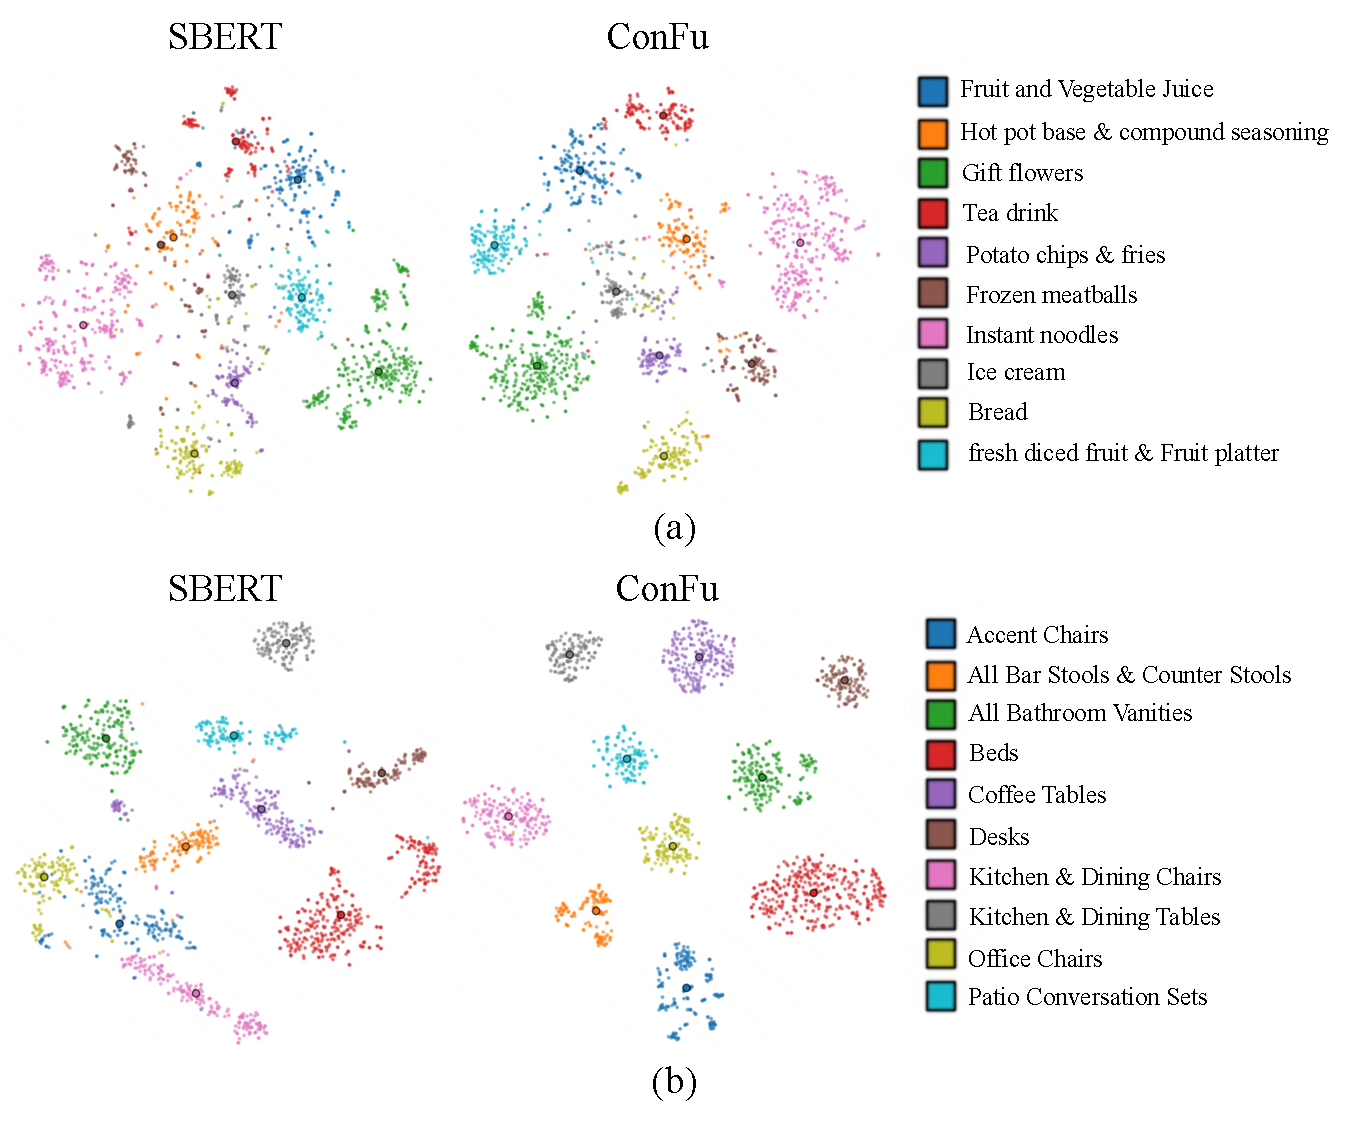
\includegraphics[width=\columnwidth]{product_vis_4}
  \caption{Product embedding visualization. (a): Product embedding visualization of MMMPS dataset. (b): Product embedding visualization of WANDS-binary dataset.}
  % \Description{A woman and a girl in white dresses sit in an open car.}
  \label{product_vis}
\end{figure}

Figure \ref{product_vis} (a) is the product embedding on MMMPS dataset. Comparing product embedding learned by SBERT and ConFu, we can see that products in MMMPS dataset are very ambiguous and ConFu can effectively inject knowledge in KG into model by optimizing product embedding based on taxonomy. 

% Besides, KGP can also optimize product embedding in some way and applying ConFu based on KGP can help model learn better product embedding, which means ConFu and KGP can complement each other. Note that although ConFu-KGP can learn the most beautiful product embedding among all six models, it does not achieve the best performance. One possible reason is that too much knowledge fusion methods cause overfitting.

% \subsubsection{Product Embedding Visualization of WANDS}

% \begin{figure*}[thbp] \centering
%   \centering
%   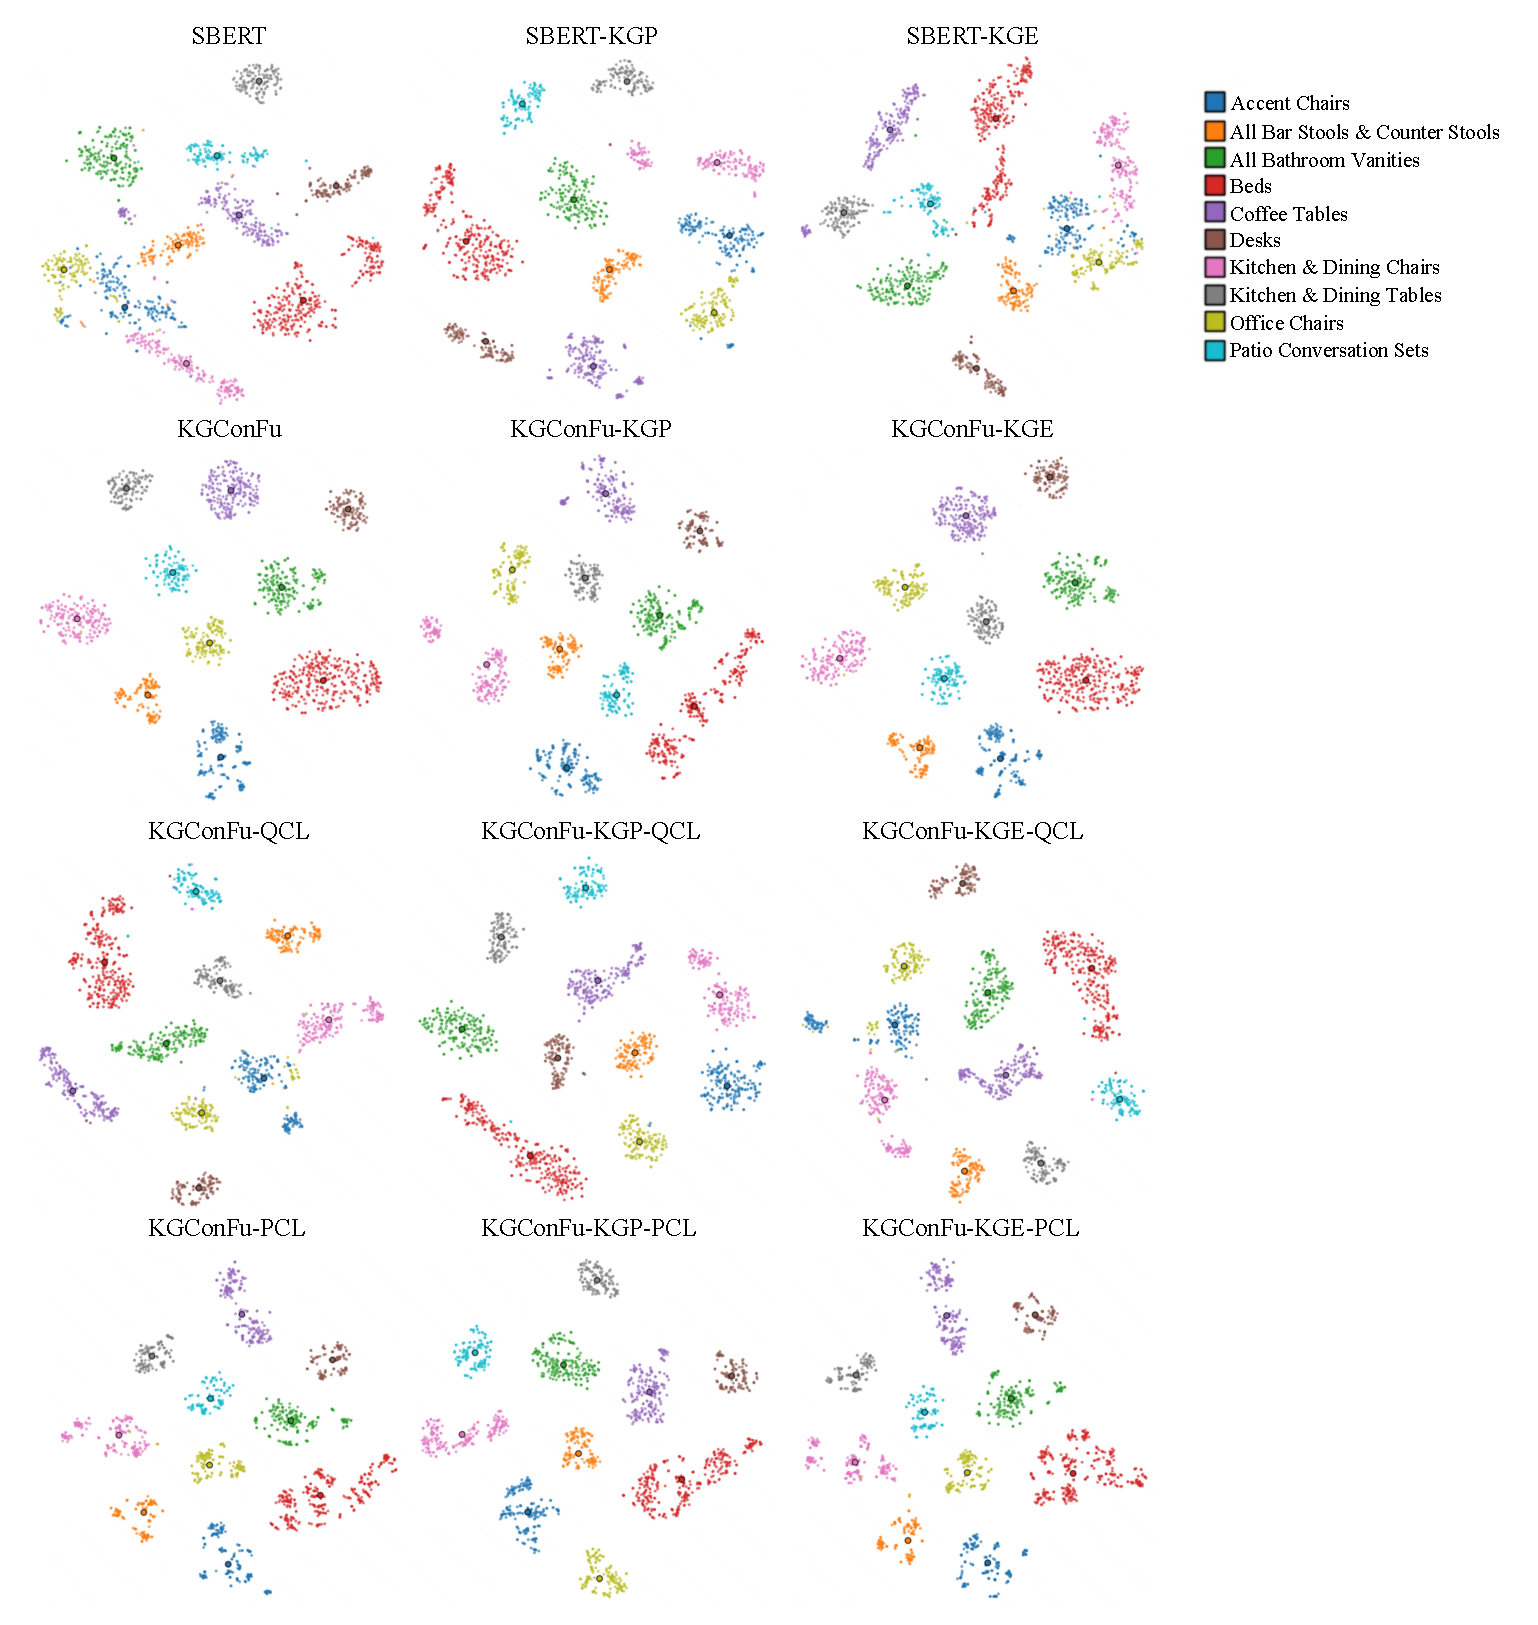
\includegraphics[width=\textwidth]{wands_product_embedding}
%   \caption{Product embedding visualization of WANDS data set.}
%   % \Description{A woman and a girl in white dresses sit in an open car.}
%   \label{wands_product_vis}
% \end{figure*}

Figure \ref{product_vis} (b) is the product embedding on WANDS-binary dataset. Different from MMMPS dataset, it is easy to see that product embedding in WANDS-binary is less ambiguous than MMMPS's and that's because most product names already contain information in taxonomy as mentioned earlier. Thus, with ConFu, products from different categories can be easily separated. This also demonstrates that PCKF is not necessary for WANDS-binary dataset. 

Generally speaking, Figure \ref{product_vis} demonstrates the ability of product embedding learning of ConFu with PCKF. In other words, taxonomy structure knowledge or relationship knowledge can be effectively fused into ConFu to some extent with PCKF.

% According to Figure \ref{wands_product_vis}, PCL can cluster products based on taxonomy, however, due to the property of the dataset itself, this kind of clustering can easily cause overfitting. Besides, according to product embedding learned by Model-QCL, QCL can also help optimize product embedding.


\subsubsection{Query Embedding Visualization of WANDS-binary}

\begin{figure}[th] 
  \centering
  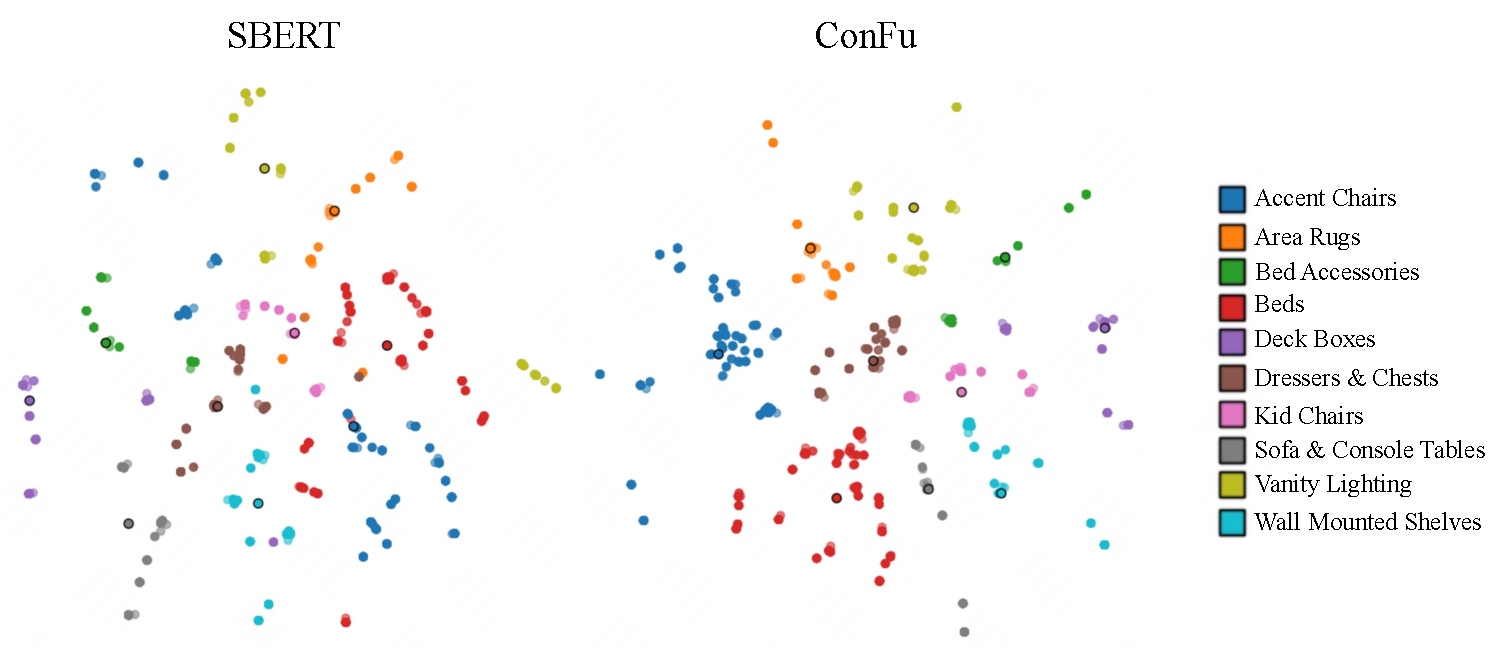
\includegraphics[width=\columnwidth]{query_vis_3}
  \caption{Query embedding visualization of WANDS-binary data set.}
  % \Description{A woman and a girl in white dresses sit in an open car.}
  \label{wands_query_vis}
\end{figure}

Figure \ref{wands_query_vis} is the query embedding on WANDS-binary dataset. According to the query embedding learned by SBERT, it is easy to see that the query embedding of WANDS-binary is chaotic. For instance, ``Accent Chair'' queries appears in both upper left corner and lower right corner in the figure. ConFu can optimize query embedding by clustering queries from the same query class, making queries with the same query class appear in the same region. Thus, for ConFu, ``Accent Chair'' queries appear in the same region in Figure \ref{wands_query_vis}.

% When QCL is removed from ConFu, PCL cannot solve the problem caused by messy query embedding, which shows the importance of QCL in ConFu on WANDS.

\subsection{Case Study}

\begin{table*}[th]
  \centering
  \setlength{\tabcolsep}{3pt}
  \begin{threeparttable}
  \caption{Case study.}
  \label{tb:case}
  \centering
  \begin{tabular}{p{3cm} p{6cm} p{6cm} p{1cm}}
    \toprule
    Query & Product & Taxonomy Path & Label \\
    \midrule
    % 蛋糕 & 奥利奥 巧轻脆薄片夹心柠檬芝士蛋糕味 95g/盒 & 0 \\
    Cake (\begin{CJK}{UTF8}{gbsn}蛋糕\end{CJK}) & Oreo Lemon Cheesecake (\begin{CJK}{UTF8}{gbsn}芝士蛋糕\end{CJK}) Flavor 95g/box & Snack Foods / Biscuit / Crispy Biscuits \& Sandwich Biscuits & 0 \\
    % \midrule
    Black-bone chicken & 4 farm Black-bone chicken eggs about 250g/serving & Raw Meat \& Raw Poultry \& Raw Eggs / Raw Eggs / Chicken Eggs & 0 \\
    % \midrule
    Sea rice (\begin{CJK}{UTF8}{gbsn}海米\end{CJK}) & About 250g dried shrimp & Seafood / Shrimp / Dried Shrimp & 1 \\
    % \midrule
    Sesame cai (\begin{CJK}{UTF8}{gbsn}芝麻菜\end{CJK}) & Stinky cai (\begin{CJK}{UTF8}{gbsn}臭菜\end{CJK}) 200g & Vegetables \& Soy Products / Leafy Vegetables / Other Leafy Vegetables & 1 \\
    Roast Duck & Vegetarian Beijing Roast Duck 100g & Snack Foods / Braised and Spicy Food / Soy Products & 0 \\
    Niuzhan (\begin{CJK}{UTF8}{gbsn}牛展\end{CJK}) & [2 catties of cooked beef tendon meat] Halal Gumei five-spice sauce marinated yellow beef leg meat ready to eat for fitness & Cooked food \& Fresh Food / Delicatessen / Braised & 1 \\
    \bottomrule
  \end{tabular}
  \begin{tablenotes}
    \item[1] Sea rice is another name of dry shrimp in Chinese.
    \item[2] Sesame cai and Stinky cai are synonyms of arugula in Chinese. Cai means ``a kind of vegetable''.
    \item[3] Niuzhan is another name of beef tendon in Chinese.
  \end{tablenotes}
  \end{threeparttable}
\end{table*}

Table \ref{tb:case} shows some bad cases that cannot be solved by baseline methods solved by ConFu on our MMMPS dataset. Note that baseline methods in this section refers to SBERT and SBERT+KGP since they have better performance. Case 1, 2 and 5 are typical examples of knowledge ignorance problem caused by lexical domination. Specifically, query exactly appears in product name, making it difficult for model to distinguish the difference between query and product. Even though taxonomy path is provided, baseline methods sometimes ignore concatenated knowledge and still cannot perfectly solve these cases, meaning the query-product case is dominated by co-occuring words. With contrastive learning, ConFu can utilize both positive and negative relationship knowledge in KG by sampling positive and negative samples from KG and learn the essence of different products, so that the problem can be alleviated. The other three cases illustrate ConFu's ability to learn synonym knowledge in KG. With QCKF and PCKF, ConFu can inject such kind of knowledge fundamentally through embedding optimization. For instance, ConFu can learn that ``Sesame cai'' and ``Stinky cai'' are two synonyms of arugula so that Case 4 can be solved. Case 3 and 6 are similar to Case 4.

% In Chinese, typos and various synonyms make PSR task more challenging. Typical knowledge fusion methods cannot fully utilize these knowlege,
